\documentclass[conference]{IEEEtran}
\IEEEoverridecommandlockouts
\usepackage{cite}
\usepackage{amsmath,amssymb,amsfonts}
\usepackage{graphicx}
\usepackage{textcomp}
\usepackage{xcolor}
\usepackage{booktabs}
\usepackage{tikz}
\usetikzlibrary{arrows.meta,positioning,fit,backgrounds,calc}

\begin{document}

\title{LabGuardian: Geometry-Constrained Pin Pose Estimation for Visual
Breadboard Reconstruction
\thanks{*Corresponding author.}}

\author{\IEEEauthorblockN{1\textsuperscript{st} Su'an Liu*}
\IEEEauthorblockA{\textit{School of Electronic Engineering}\\
\textit{Beijing University of Posts}\\
\textit{and Telecommunications}\\
Beijing, China\\
buptliusuan@gmail.com}
\and
\IEEEauthorblockN{2\textsuperscript{nd} Xinran Zhang}
\IEEEauthorblockA{\textit{School of Electronic Engineering}\\
\textit{Beijing University of Posts}\\
\textit{and Telecommunications}\\
Beijing, China\\
% TODO(author): insert institutional email or ORCID before submission
}
\and
\IEEEauthorblockN{3\textsuperscript{rd} Jiali Ruan}
\IEEEauthorblockA{\textit{School of Electronic Engineering}\\
\textit{Beijing University of Posts}\\
\textit{and Telecommunications}\\
Beijing, China\\
% TODO(author): insert institutional email or ORCID before submission
}
}

\maketitle

\begin{abstract}
Recovering the wiring of a breadboard circuit from a single photograph is a
fine-grained visual structure problem: holes are separated by a 2.54 mm pitch,
component terminals are thin and frequently occluded, and a displacement of one
grid cell changes the inferred electrical connection. Component detectors stop
at bounding boxes and cannot say which hole a lead enters, whereas end-to-end
multimodal models may describe a plausible topology that the image does not
support. We present LabGuardian, a vision pipeline that formulates terminal
localization as component-conditioned pose estimation. A full-frame
keypoint model predicts component instances together with ordered terminal
keypoints, a planar homography rectifies the board to a canonical metric plane,
and a geometry-constrained snap-to-grid stage maps each rectified terminal to a
discrete hole under package and board feasibility constraints while retaining
ranked alternatives for ambiguous terminals. Every downstream relation stays
linked to its originating instance, keypoint and candidate hole, so the
reconstruction is auditable rather than asserted. On a disjoint validation split, component
detection reaches 0.991 mAP50 and 0.786 mAP50-95 and pin pose estimation reaches
0.947 and 0.829. INT8 execution on an Intel Core Ultra 5 225U neural processing
unit runs at 13.37 ms mean latency, 15.61 ms at the 99th percentile and 74.7
images per second within 8.53 W package power.
\end{abstract}

\begin{IEEEkeywords}
pose estimation, keypoint localization, homography, visual circuit
reconstruction, edge inference
\end{IEEEkeywords}

\section{Introduction}

Converting a photograph of a physical circuit into an explicit structural
description is a prerequisite for automated inspection of hand-wired hardware,
for robotic assembly verification, and for assistive systems that check a
prototype against an intended design. Breadboards make this problem concrete
and unusually strict. Holes are arranged on a regular 2.54 mm lattice, and the
electrical meaning of a component is determined entirely by which holes its
terminals occupy. Two reconstructions that differ by a single grid cell describe
different circuits: one may be the intended amplifier, the other an open loop or
an unintended short. Accuracy therefore has to be defined at the level of
individual holes rather than of component bodies.

Most visual pipelines stop before that level. A detector that returns a box
labeled \emph{resistor} identifies the presence of a device but not where its
leads enter the board, and cropping the box before regressing terminals removes
exactly the evidence needed: axial leads extend well beyond the component body,
and the surrounding lattice provides the reference against which a terminal
position becomes meaningful. The natural representation is an
instance-conditioned set of terminal keypoints predicted in the full image.

A second difficulty is geometric rather than semantic. Nearest-neighbor
matching in image coordinates is not invariant to viewpoint: under an oblique
camera the row spacing compresses, and a terminal can be attracted to the wrong
row even when its pixel localization is correct. Purely learned image-to-topology
models, in turn, have no explicit mechanism to enforce the planar lattice, the
separation across the central trench, the span of an axial device, or the pin
order of a dual in-line package. Multimodal language models provide flexible
visual semantics~\cite{llava}, but a free-form description cannot guarantee that
a claimed connection corresponds to observed pixels; we refer to such
unsupported structural statements as \emph{topology hallucination}. In a
verification setting this failure mode is worse than a missed detection, because
an unsupported claim is indistinguishable from a supported one.

LabGuardian therefore treats reconstruction as a sequence of visual estimation
and geometric projection steps, each of which produces an inspectable
intermediate result. A full-frame pose network predicts component instances and
ordered terminal keypoints; a planar homography maps the board to a canonical
metric plane; and a geometry-constrained snap-to-grid stage converts rectified
coordinates into discrete hole hypotheses, keeping ranked alternatives wherever
the observation does not support a unique assignment. Electrical interpretation
and symbolic comparison consume this pin-hole graph but never modify it, so a
structural conclusion can always be traced back to a bounding box, a keypoint, a
rectified coordinate and a candidate hole.

The contributions of this paper are as follows.

\begin{itemize}
\item We formulate terminal localization as component-conditioned pose
estimation on the full board image, and associate pin hypotheses with component
instances through a multi-cue, category-gated matching score with explicit
abstention.
\item We introduce a projective-to-discrete geometric interface that couples
homography-based rectification with a feasibility-constrained snap-to-grid
assignment, and that represents residual hole-level ambiguity explicitly
instead of resolving it silently.
\item We report accuracy and heterogeneous edge inference for the complete
visual stage: 0.947 pin mAP50 and 0.829 pin mAP50-95, and 13.37 ms mean latency
at 74.7 images per second within 8.53 W on an integrated neural processing unit.
\end{itemize}

\section{Related Work}

\subsection{Keypoint and Pose Estimation}

Pose estimation maps an image to structured landmarks instead of a category or a
box. High-resolution architectures such as HRNet improve spatial precision by
maintaining multi-scale feature streams throughout the
network~\cite{hrnet}, while single-stage formulations such as YOLO-Pose regress
boxes and keypoints jointly and retain instance-level grouping in one forward
pass~\cite{yolopose,yolo}. We adopt this heatmap-free family but reinterpret the
pose: the instance is a rigid electronic component and the landmarks are its
electrical terminals. Unlike human joints, these landmarks are small, often
collinear, and constrained both by package geometry and by the regular lattice
that receives them, which makes the surrounding context at least as informative
as the appearance of the instance itself.

\subsection{Planar Rectification and Metric Grids}

Projective rectification of a plane from four correspondences is a standard tool
for normalizing viewpoint~\cite{hartley,zhangcalib}. A breadboard is a
favorable case, since its working surface is approximately planar and carries a
repeated metric grid that provides landmarks. Rectification alone, however, does
not decide between two adjacent holes when a terminal projects near their
common boundary. Our contribution at this stage is not the homography itself but
its coupling to a discrete assignment layer that encodes board topology, package
type, terminal span, collinearity and trench separation, and that reports the
constraint responsible for each rejection.

\subsection{Circuit Understanding and Symbolic Verification}

Work on circuit data has largely addressed schematic-level recognition, printed
circuit board inspection, or already symbolic netlists~\cite{amsnet}. Simulation
and graph matching operate on a symbolic circuit that is assumed to be
available~\cite{spice,vf2}, and language-model approaches to electronic design
consume textual or structural descriptions rather than raw
photographs~\cite{llm4eda}. Conversely, generic multimodal models summarize
visual content without providing a deterministic pixel-to-hole correspondence.
The interface between these regimes, namely the recovery of terminals and their
canonical board locations from a photograph, is the gap addressed here. Symbolic
comparison is retained in our system only as a downstream consumer of the visual
reconstruction and is not claimed as a contribution.

\section{Method}

\subsection{Problem Formulation}

Let an RGB image $I \in \mathbb{R}^{H \times W \times 3}$ show component
instances $\mathcal{C}=\{C_i\}$. Each instance carries a class $t_i$, a
bounding box $b_i$, and an ordered set of terminal keypoints
$K_i=\{\mathbf{p}_{ik}\}$ with visibility flags. A board model supplies canonical
hole centers $\mathcal{H}=\{\mathbf{c}_h\}$ together with feasibility relations
induced by the board layout and by component packaging. The task is to estimate
\begin{equation}
F: I \longrightarrow \{(C_i,\, k,\, h,\, z_{ik})\},
\label{eq:task}
\end{equation}
where $h$ is the assigned hole and $z_{ik}$ records keypoint confidence,
rectified projection distance, candidate rank, visibility and an ambiguity flag.
The formulation deliberately precedes electrical interpretation: it states what
the image supports, not whether the circuit is correct. Fig.~\ref{fig:pipeline}
summarizes the resulting stages.

\begin{figure}[!t]
\centering
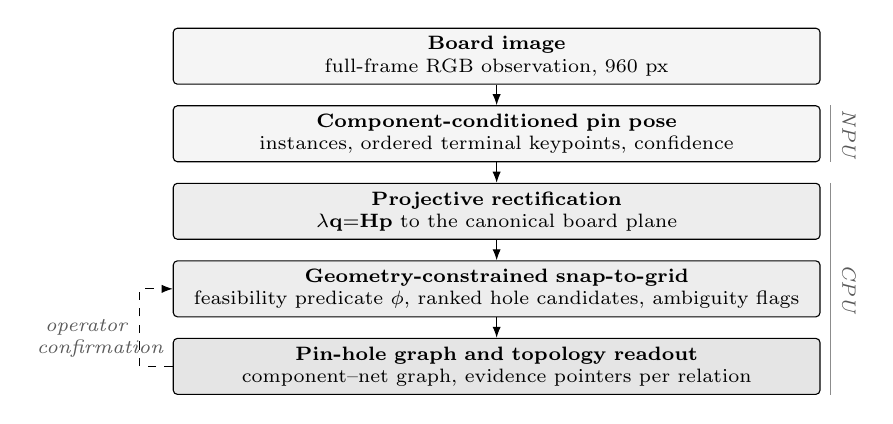
\begin{tikzpicture}[
  font=\scriptsize,
  box/.style={draw, rounded corners=1.5pt, align=center, inner sep=3pt,
              text width=0.66\columnwidth, line width=0.4pt},
  vis/.style={box, fill=black!4},
  geo/.style={box, fill=black!7},
  sym/.style={box, fill=black!10},
  ar/.style={-{Latex[length=1.4mm]}, line width=0.4pt},
  unit/.style={font=\scriptsize\itshape, text=black!65}
]
\node[vis] (img) {\textbf{Board image}\\full-frame RGB observation, 960 px};
\node[vis, below=2.6mm of img] (pose)
  {\textbf{Component-conditioned pin pose}\\instances, ordered terminal
   keypoints, confidence};
\node[geo, below=2.6mm of pose] (rect)
  {\textbf{Projective rectification}\\$\lambda\mathbf{q}{=}\mathbf{H}\mathbf{p}$ to the canonical board plane};
\node[geo, below=2.6mm of rect] (snap)
  {\textbf{Geometry-constrained snap-to-grid}\\feasibility predicate $\phi$,
   ranked hole candidates, ambiguity flags};
\node[sym, below=2.6mm of snap] (graph)
  {\textbf{Pin-hole graph and topology readout}\\component--net graph,
   evidence pointers per relation};

\draw[ar] (img) -- (pose);
\draw[ar] (pose) -- (rect);
\draw[ar] (rect) -- (snap);
\draw[ar] (snap) -- (graph);

\draw[line width=0.4pt, black!45]
  ($(pose.north east)+(1.3mm,0)$) -- ($(pose.south east)+(1.3mm,0)$);
\node[unit, rotate=-90, anchor=center] at ($(pose.east)+(3.6mm,0)$) {NPU};
\draw[line width=0.4pt, black!45]
  ($(rect.north east)+(1.3mm,0)$) -- ($(graph.south east)+(1.3mm,0)$);
\node[unit, rotate=-90, anchor=center] at ($(snap.east)+(3.6mm,0)$) {CPU};

\draw[ar, dashed, line width=0.35pt]
  (graph.west) -- ++(-0.42,0) |- (snap.west);
\node[align=center, font=\scriptsize\itshape, text=black!65, text width=1.25cm]
  at ($(graph.west)+(-1.1,0.35)$) {operator\\confirmation};
\end{tikzpicture}
\caption{Visual reconstruction pipeline. Perception, rectification and discrete
assignment are separated so that every stage can be inspected independently.
Topology readout consumes the pin-hole graph but does not alter the visual
observations; a confirmed hole assignment re-runs only the geometric and
symbolic stages. Vertical rules on the right indicate the execution unit that
hosts each stage on the target platform.}
\label{fig:pipeline}
\end{figure}

\subsection{Component-Conditioned Pin Pose Estimation}

The pose network processes the complete image at 960 px resolution and, for
every detected component, regresses a box, a class score, terminal coordinates,
per-keypoint visibility and per-keypoint confidence. Full-frame inference is a
deliberate choice: it preserves leads that leave the component body and the
lattice that surrounds them, both of which a crop would discard. Seven classes
are annotated directly: resistor, ceramic capacitor, electrolytic capacitor,
diode, light-emitting diode, jumper wire and three-terminal transistor. Dense
dual in-line packages are treated differently. Their pins occupy only a few
pixels each and direct keypoint regression is unstable, so pin positions are
derived from rigid package geometry once the package and its orientation have
been detected.

Component and pose hypotheses are produced by two heads and must be associated
before a netlist can be built; a terminal claimed by a neighboring device
propagates into a wrong electrical relation. For component $i$ and pose
hypothesis $j$ we compute
\begin{equation}
\begin{split}
S_{ij} = {} & w_1\,\mathrm{IoU}(b_i,b_j)
  + w_2 \exp\!\left(-\frac{\lVert \boldsymbol{\mu}_i-\boldsymbol{\mu}_j
    \rVert_2^2}{2\sigma_i^2}\right)\\
  & + w_3\,\rho_{ij} + w_4\,\gamma_{ij} + w_5\,c_j,
\end{split}
\label{eq:association}
\end{equation}
where $\boldsymbol{\mu}$ denotes a box center, $\rho_{ij}$ is the fraction of
keypoints falling inside a dilated component box, $\gamma_{ij}$ measures the
consistency between keypoint span and component extent, and $c_j$ is the
detection confidence. Pairs with incompatible classes are removed, the remaining
pairs are sorted by $S_{ij}$ and assigned greedily one to one, so a terminal
cannot be owned twice. If the best score of a pose hypothesis falls below an
acceptance threshold, the hypothesis is left unmatched and flagged rather than
attached to the closest device. Abstention is preferred here because an
unmatched terminal is visible to an operator, whereas a wrong owner silently
corrupts the netlist.

\begin{figure*}[!t]
\centering
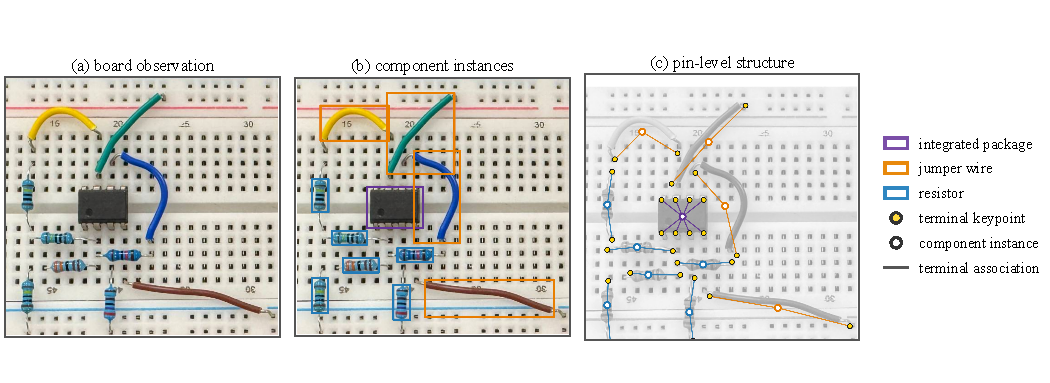
\includegraphics[width=0.98\textwidth]{figures/en/reconstruction.pdf}
\caption{Reconstruction on a real board. (a) full-frame observation; (b)
component instances with class-coded boxes; (c) the instance-linked pin
representation after geometric mapping, where each terminal keypoint is bound to
a component node and to the hole it occupies. Panel (c) is the interface consumed
by topology readout; it adds no visual evidence of its own.}
\label{fig:reconstruction}
\end{figure*}

\subsection{Projective Rectification}

Let $\mathbf{p}=[x_p,y_p,1]^\top$ be a terminal keypoint in image coordinates.
Four board landmarks determine a nonsingular planar homography
$\mathbf{H}\in\mathbb{R}^{3\times 3}$, and the canonical coordinate
$\mathbf{q}=[u,v,1]^\top$ follows from
\begin{equation}
\begin{split}
\lambda\mathbf{q} &= \mathbf{H}\mathbf{p},\\
u &= \frac{h_{11}x_p+h_{12}y_p+h_{13}}{h_{31}x_p+h_{32}y_p+h_{33}},\qquad
v = \frac{h_{21}x_p+h_{22}y_p+h_{23}}{h_{31}x_p+h_{32}y_p+h_{33}},
\end{split}
\label{eq:homography}
\end{equation}
with $\lambda\neq 0$ the homogeneous scale and $h_{ij}$ the entries of
$\mathbf{H}$. Equation~\eqref{eq:homography} removes projective distortion
before any discrete decision is taken, which makes the acceptance radius of the
next stage a physical quantity instead of a viewpoint-dependent one. When
landmark calibration fails, a synthetic lattice is used as a fallback, but every
assignment produced under the fallback is marked so that it is not treated as
equally reliable evidence.

\subsection{Geometry-Constrained Snap-to-Grid}

Given the rectified coordinate and the canonical hole set, the candidate
assignment and its acceptance rule are
\begin{align}
h^{*} &= \arg\min_{h\in\mathcal{H}}
   \lVert \mathbf{q}_{1:2}-\mathbf{c}_h \rVert_2,
   \qquad a = \frac{d_{h^{*}}}{s_g},
\label{eq:snap}\\
\mathrm{accept} &= (a \le \tau) \wedge
   \bigl(\phi(h^{*},t_p,K_i)=1\bigr),
\label{eq:accept}
\end{align}
where $d_{h^{*}}$ is the rectified snapping distance, $s_g$ the physical grid
pitch, $\tau$ a normalized threshold, $t_p$ the terminal or package type, and
$\phi$ a feasibility predicate. The predicate rejects assignments that leave the
board region, cross the central trench where the two halves are electrically
separate, violate the span of an axial device, break the collinearity of a
three-terminal device, or contradict package-specific pin order. Normalizing the
snapping distance by $s_g$ in~\eqref{eq:snap} makes $\tau$ independent of output
resolution.

Rejection does not discard the observation. The mapper records the ranked
candidate holes, their normalized distances, the violated constraint and a
confidence flag, so a terminal that projects near the boundary between two holes
is reported as ambiguous rather than resolved by an arbitrary tie-break
(Fig.~\ref{fig:ambiguity}). This is a deliberate design decision: dense
millimeter-scale holes are an intrinsically hard localization target, a residual
hole-level error cannot be driven to zero by a stronger backbone alone, and a
sub-pixel residual that is silently rounded becomes a false structural claim.
Where a low-confidence assignment matters, a single operator confirmation
resolves it and only the geometric and symbolic stages are recomputed; the
perception result is not discarded.

\begin{figure}[!t]
\centering

\includegraphics[width=0.98\columnwidth]{figures/en/ambiguity.pdf}
\caption{Hole-level ambiguity. (a) A terminal that projects between adjacent
holes is retained as several ranked candidates with their scores instead of being
forced onto the nearest one. (b) After confirmation the terminal is bound to a
single hole and the downstream graph is recomputed without re-running
perception.}
\label{fig:ambiguity}
\end{figure}

\subsection{Topology Readout}

Accepted pin-hole relations are grouped into electrical nodes using the known
breadboard layout, in which each five-hole strip is internally connected and the
power rails span the board. A disjoint-set structure merges the strips joined by
detected jumper wires, and the result is a component--net graph in which nets are
nodes and non-wire components are edges. Physical holes remain the only source of
node identity, so a corrected hole assignment regenerates node labels instead of
inheriting stale ones.

The graph can be exported as a topology-level netlist and compared against a
reference by subgraph isomorphism~\cite{vf2}, which yields structured mismatch
codes. These operations add no visual evidence and are not evaluated as part of
our claims; their role is to test whether the reconstructed structure is usable
downstream. Because each mismatch retains pointers to the originating instance,
keypoint, rectified coordinate and candidate hole, a conclusion can be audited
back to the pixels that produced it.

\section{Experiments}

\subsection{Implementation and Data}

Experiments use a private dataset of real top-view breadboard photographs
covering six textbook analog circuit topologies: a first-order RC network, a
common-emitter amplifier, a differential pair, and inverting, integrating and
summing amplifiers built around a general-purpose operational amplifier. The
images were captured under varying viewpoint and illumination and include wire
overlap and partial occlusion, so no synthetic augmentation of the scene layout
was required. Annotations combine component boxes with up to three ordered
terminal keypoints per instance and per-keypoint visibility. Training,
validation and test splits are disjoint, and the test split is excluded from
optimization and model selection.
% TODO(author): insert per-split image, instance and keypoint counts from the
% training manifest before submission.

The pose model is YOLOv8s-pose~\cite{yolo}, trained for 100 epochs at 960 px
input with batch size 8, standard color, translation and scale augmentation, and
mosaic augmentation disabled for the final ten epochs. Post-training INT8
quantization used 144 calibration images and reduced the exported model from
22 MB to 11 MB. All deployment measurements were taken on an edge platform built
around an Intel Core Ultra 5 225U with 8 GB of memory, which exposes CPU,
integrated GPU and neural processing unit execution paths through a common
runtime~\cite{intel225u,openvino}. Between 60 and 1153 serial inferences were
collected per configuration, and package power was sampled from the running
average power limit interface at 0.25 s intervals.

\subsection{Detection and Pin Pose Accuracy}

Table~\ref{tab:accuracy} reports validation accuracy after 100 epochs. The
keypoint head keeps precision and recall above 0.95 despite the small spatial
support of a terminal, which indicates that terminals of the annotated classes
are reliably found and attributed to the correct instance. The gap between pin
mAP50 and mAP50-95 is the more informative number for our purpose: coarse
keypoint detection is largely solved, while strict localization is not, and it is
precisely the strict regime that determines whether a terminal falls on the
correct side of a hole boundary. This is the empirical motivation for treating
rectification and constrained assignment as separate, inspectable stages rather
than expecting the pose head to resolve hole identity by itself.

\begin{table}[!t]
\caption{Validation accuracy after 100 epochs}
\label{tab:accuracy}
\centering
\begin{tabular}{lcccc}
\toprule
Prediction target & Precision & Recall & mAP50 & mAP50-95 \\
\midrule
Component boxes & 0.991 & 0.989 & 0.991 & 0.786 \\
Pin keypoints   & 0.955 & 0.954 & 0.947 & 0.829 \\
\bottomrule
\end{tabular}
\end{table}

\subsection{Heterogeneous Edge Inference}

Table~\ref{tab:devices} lists latency and throughput for the six
device--precision configurations. INT8 execution on the neural processing unit
attains the lowest mean and tail latency, reducing mean latency by 85.5\%
relative to CPU FP16 and raising throughput from 60.4 to 74.7 images per second
relative to FP16 on the same unit. The 15.61 ms 99th-percentile latency is the
relevant figure for interactive use, since it bounds the delay of the visual
stage rather than its average cost.

\begin{table}[!t]
\caption{Latency and throughput of the pose model across execution units}
\label{tab:devices}
\centering
\setlength{\tabcolsep}{3.6pt}
\begin{tabular}{llccccc}
\toprule
Device & Prec. & Load (s) & Mean (ms) & P95 (ms) & P99 (ms) & img/s \\
\midrule
CPU  & FP16 & 0.14 & 92.44 & 96.74 & 98.92 & 10.8 \\
CPU  & INT8 & 0.24 & 29.02 & 30.13 & 30.65 & 34.5 \\
iGPU & FP16 & 0.43 & 26.87 & 27.32 & 28.18 & 37.2 \\
iGPU & INT8 & 2.85 & 18.26 & 19.29 & 20.11 & 54.7 \\
NPU  & FP16 & 1.01 & 16.55 & 16.64 & 17.67 & 60.4 \\
\textbf{NPU} & \textbf{INT8} & \textbf{1.20} & \textbf{13.37} &
\textbf{13.75} & \textbf{15.61} & \textbf{74.7} \\
\bottomrule
\end{tabular}
\end{table}

Fig.~\ref{fig:power} shows the package power trace of the three INT8
configurations measured in one session. Two observations follow. First, the
neural processing unit sustains the workload at 8.53 W package power, roughly
4.1 W above the 4.4 W idle baseline. This corresponds to 114.2 mJ per inference,
or 18.1 images per second per watt of incremental power, whereas the CPU
configuration draws 26.4 W at 34.5 images per second and therefore spends
roughly seven times more energy on the same inference. Second, during neural
processing unit execution the CPU-core and integrated-GPU power curves stay near
their idle level, so the units are genuinely free for other work. This is what
makes the division of labor in Fig.~\ref{fig:pipeline} practical on one 8 GB
platform: perception is resident on the neural processing unit while graph
construction, rectification bookkeeping and verification run on the CPU.

\begin{figure}[!t]
\centering
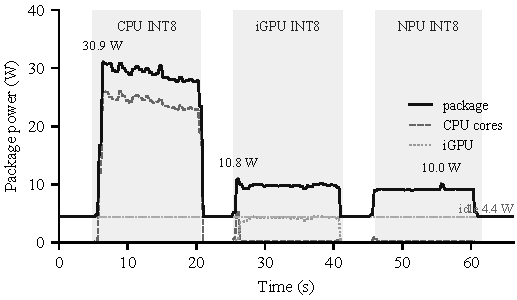
\includegraphics[width=0.98\columnwidth]{figures/en/power.pdf}
\caption{Package power during three INT8 inference phases on the same platform.
Peak package power is annotated per phase. While the neural processing unit is
loaded, CPU-core and integrated-GPU power remain at the idle baseline.}
\label{fig:power}
\end{figure}

\subsection{Qualitative Analysis}

Fig.~\ref{fig:reconstruction} shows a complete reconstruction. Boxes and classes
are recovered on a cluttered board, and the pin-level panel makes explicit which
terminal belongs to which instance and which hole each terminal occupies. Two
failure sources are visible in this representation and are worth separating.
Component boxes can be correct while terminal endpoints are partially hidden by
jumper wires, and full-frame inference is what preserves the visible lead
direction and neighboring lattice needed to place such endpoints. Independently,
a terminal can be localized accurately and still fall near a boundary between
two holes after rectification, as in Fig.~\ref{fig:ambiguity}; this is a
geometric condition, not a perception error, and the pipeline reports it as such.

\begin{figure*}[!t]
\centering
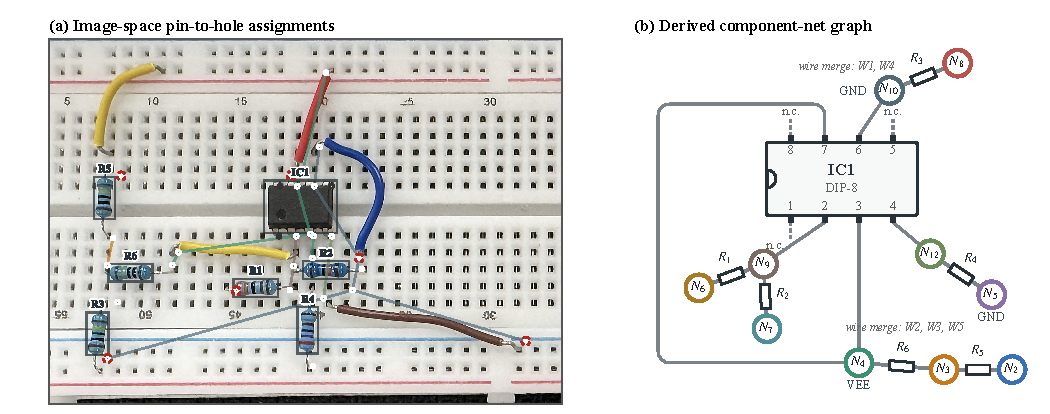
\includegraphics[width=0.96\textwidth]{figures/en/netlist.pdf}
\caption{Topology readout for the board of Fig.~\ref{fig:reconstruction}: 11
components, 28 terminals and 10 electrical nodes. (a) Terminals bound to holes,
with one color per electrical node and jumper wires merged into their nodes.
(b) The resulting component--net graph, in which nets are nodes and non-wire
components are edges. Node identity comes from physical holes, so a corrected
assignment regenerates the graph.}
\label{fig:netlist}
\end{figure*}

Fig.~\ref{fig:netlist} shows the structure obtained from the same board after
grouping: 11 components and 28 terminals resolve into 10 electrical nodes, with
power and ground rails distinguishable from signal nodes. The example is included
as evidence that the visual output is complete enough to be consumed
symbolically, not as a claim about diagnostic accuracy. On this platform the
deterministic path from a rectified pose result to a topology comparison
completes in under 100 ms, so the visual stage dominates the end-to-end cost.

\subsection{Cost of the Auditable Interface}

Keeping perception, geometry and interpretation separate has an engineering
cost, which we report for completeness. An optional on-device explanation module,
used to verbalize structured findings under the fixed evidence produced by the
symbolic stage, occupies 941.5 MB after INT4 weight compression, down from
3.1 GB, and peaks at 1.36 GB resident memory with 63.9 ms to the first token and
23.2 tokens per second on the integrated GPU~\cite{qwen25,lora,openvino-int4}.
It therefore coexists with the vision model inside the 8 GB budget. Because this
module only rephrases findings it is given and cannot alter the reconstruction,
it is outside the scope of the visual claims evaluated above.

\section{Discussion and Limitations}

The results above quantify the perception stage and the cost of deploying it:
terminals of the annotated classes are localized and attributed accurately, and
the visual stage runs at interactive rates within an embedded power budget. The
geometric stage is evaluated qualitatively here, and a quantitative hole-level
benchmark remains open. Reporting pin-to-hole assignment accuracy, or an ablation
that separates projective rectification from unconstrained nearest-neighbor
snapping, requires per-terminal hole labels that the present annotation does not
carry, and we prefer to state the protocol rather than approximate it from pose
average precision: normalized keypoint error and PCK for the continuous stage,
hole-assignment accuracy after rectification and snapping for the discrete
stage, ambiguity-rejection precision over the terminals rejected by $\phi$, each
stratified by viewpoint obliquity and occlusion level. Collecting these labels
for a held-out subset is the next step, and it is what would isolate the
contribution of the geometric layer from that of the pose model.

Two further limitations bound the present results. The dataset is private and its
keypoints denote rigid terminals rather than articulated joints, so results are
not directly comparable with public pose benchmarks; releasing the annotations
and the board geometry would improve reproducibility more than any additional
architectural change. And the symbolic stage can detect that a reconstruction is
structurally inconsistent with a reference, but it cannot certify that an
individual keypoint or hole assignment was correct. Visual and structural
metrics must therefore continue to be reported separately, which is also why the
system exposes ambiguity to an operator instead of resolving it internally.

\section{Conclusion}

We presented LabGuardian, which reframes breadboard understanding as pin-level
pose estimation coupled to an explicit geometric interface. Full-frame,
component-conditioned keypoint prediction preserves the lead and lattice context
that cropping destroys; a planar homography maps arbitrary viewpoints to a
canonical board; and a feasibility-constrained snap-to-grid stage converts
rectified coordinates into discrete hole hypotheses while keeping residual
ambiguity visible. The reconstruction is auditable because every downstream
relation remains bound to the image evidence that produced it. Validation
accuracy and cross-device measurements show that the approach is spatially
accurate at the pose level and suitable for real-time execution on an integrated
neural processing unit. The immediate next step is the controlled geometric
ablation and the pin-to-hole benchmark described above, which are required to
quantify the geometric stage independently of the pose model.

\begin{thebibliography}{00}
\bibitem{llava} H. Liu, C. Li, Q. Wu, and Y. J. Lee, ``Visual instruction
tuning,'' in \emph{Advances in Neural Information Processing Systems}, vol. 36,
2023, pp. 34892--34916.
\bibitem{hrnet} K. Sun, B. Xiao, D. Liu, and J. Wang, ``Deep high-resolution
representation learning for human pose estimation,'' in \emph{Proc. IEEE/CVF
Conf. Computer Vision and Pattern Recognition}, 2019, pp. 5693--5703.
\bibitem{yolopose} D. Maji, S. Nagori, M. Mathew, and D. Poddar, ``YOLO-Pose:
enhancing YOLO for multi person pose estimation using object keypoint similarity
loss,'' in \emph{Proc. IEEE/CVF Conf. Computer Vision and Pattern Recognition
Workshops}, 2022, pp. 2637--2646.
\bibitem{yolo} G. Jocher, A. Chaurasia, and J. Qiu, ``Ultralytics YOLOv8,''
2023. [Online]. Available: https://docs.ultralytics.com
\bibitem{hartley} R. Hartley and A. Zisserman, \emph{Multiple View Geometry in
Computer Vision}, 2nd ed. Cambridge, U.K.: Cambridge Univ. Press, 2003.
\bibitem{zhangcalib} Z. Zhang, ``A flexible new technique for camera
calibration,'' \emph{IEEE Trans. Pattern Anal. Mach. Intell.}, vol. 22, no. 11,
pp. 1330--1334, 2000.
\bibitem{amsnet} Y. Shi, Z. Tao, Y. Gao, T. Zhou, C. Chang, Y. Wang, B. Chen,
G. Zhang, S. Liu, Z. Yu, T.-J. Lin, and L. He, ``AMSnet 2.0: a large AMS database
with AI segmentation for net detection,'' arXiv:2505.09155, 2025.
\bibitem{spice} L. W. Nagel, ``SPICE2: a computer program to simulate
semiconductor circuits,'' Ph.D. dissertation, Univ. California, Berkeley, CA,
USA, 1975.
\bibitem{vf2} L. P. Cordella, P. Foggia, C. Sansone, and M. Vento, ``A
(sub)graph isomorphism algorithm for matching large graphs,'' \emph{IEEE Trans.
Pattern Anal. Mach. Intell.}, vol. 26, no. 10, pp. 1367--1372, 2004.
\bibitem{llm4eda} R. Zhong, X. Du, S. Kai, Z. Tang, S. Xu, H.-L. Zhen, J. Hao,
Q. Xu, M. Yuan, and J. Yan, ``LLM4EDA: emerging progress in large language models
for electronic design automation,'' arXiv:2401.12224, 2024.
\bibitem{intel225u} Intel Corporation, ``Intel Core Ultra 5 processor 225U
specifications,'' 2025. [Online]. Available:
https://www.intel.com/content/www/us/en/products/sku/241861
\bibitem{openvino} Intel Corporation, ``OpenVINO toolkit documentation,'' 2024.
[Online]. Available: https://docs.openvino.ai
\bibitem{qwen25} Qwen Team, ``Qwen2.5 technical report,'' arXiv:2412.15115,
2024.
\bibitem{lora} E. J. Hu, Y. Shen, P. Wallis, Z. Allen-Zhu, Y. Li, S. Wang,
L. Wang, and W. Chen, ``LoRA: low-rank adaptation of large language models,'' in
\emph{Proc. Int. Conf. Learning Representations}, 2022.
\bibitem{openvino-int4} Intel Corporation, ``4-bit weight quantization,''
OpenVINO documentation, 2024. [Online]. Available: https://docs.openvino.ai
\end{thebibliography}

\end{document}
